\begin{table*}[t]
\centering
\small
\resizebox{0.99\textwidth}{!}{
\begin{tabular}{l|c|c|c|c|c|c}
\toprule
  % & & \multicolumn{3}{c|}{Simulation Benchmark (\# tasks)} & \\
  Method & Params (M) & Modality & Adroit (3)~\cite{rajeswaran2017learning} & DexArt (4)~\cite{bao2023dexart} & Bi-DexHands (4)~\cite{chen2023bi} & Average Success  \\
\midrule
  Diffusion Policy~\cite{chi2023diffusion} & 266.8 & 2D & \dd{0.32}{0.03} & \dd{0.49}{0.04} & \dd{0.42}{0.05} & \dd{0.42}{0.04} \\
  HPT~\cite{wang2024scaling} & 13.99 & 2D & \dd{0.45}{0.02}  & \dd{0.53}{0.05} & \dd{0.44}{0.04} & \dd{0.47}{0.04}  \\
  UniAct~\cite{zheng2025universal} & 1053 & 2D & \dd{0.49}{0.01} & \dd{0.55}{0.03} & \dd{0.47}{0.07} & \dd{0.50}{0.05} \\
  
  3D Diffusion Policy~\cite{ze20243d} & 255.2 & 3D & \dd{0.68}{0.03} & \dd{0.69}{0.02} & \dd{0.55}{0.14} & \dd{0.63}{0.06} \\
  3D ManiFlow Policy~\cite{yan2025maniflow} & 218.9 & 3D & \dd{0.70}{0.02} & \dd{0.70}{0.03} & \dd{0.59}{0.07} & \dd{0.66}{0.04} \\
  \textbf{\mymethod{} (Ours)} & 19.36 & 3D & \ddbfgreen{0.75}{0.02} & \ddbfgreen{0.73}{0.03} & \ddbfgreen{0.67}{0.05} & \ddbfgreen{0.71}{0.04} \\
\bottomrule

% {\cellcolor{tablecolor2}$\mathbf{0.72}$}  \\

\end{tabular}
}
\vspace{-8pt}
\caption{Quantitative comparison of our method against 2D (image-based) and 3D (point cloud-based) baselines on 11 dexterous manipulation tasks from the Adroit~\cite{rajeswaran2017learning}, DexArt~\cite{bao2023dexart}, and Bi-DexHands~\cite{chen2023bi} simulation benchmarks.}
\vspace{-16pt}
\label{tab:sim}
\end{table*}

\vspace{-4pt}
\section{Experiments}
\vspace{-2pt}
\label{sec:experiments}

\subsection{Datasets and Experimental Setup}

% \subsubsection{Offline Pre-training Datasets}
\noindent\textbf{Offline Pre-training Datasets.}
Our approach leverages large-scale, heterogeneous datasets for pre-training. 
The full dataset is a mixture from three distinct sources, as detailed in Figure~\ref{fig:dataset_count}. For \textbf{human demonstrations}, we use HOI4D~\cite{liu2022hoi4d}, Ego-Exo4D~\cite{grauman2024ego} and Aria Digital Twin (ADT)~\cite{pan2023aria}, which include large-scale 4D egocentric dataset of human-object interactions. We leverage its 3D point cloud observations and corresponding MANO hand poses. To integrate this data, we process the MANO model parameters to generate our structural action representation $\mathbf{A} \in \mathbb{R}^{D_a \times T}$ and tag each joint according to our Embodied Joint Codebook (same for Robot and Simulation). For \textbf{robot demonstrations}, we incorporate 3D dexterous manipulation data from existing robot datasets, including Fourier ActionNet~\cite{fourier2025actionnet} and DexCap~\cite{wang2024dexcap}, which provide diverse 3D interaction trajectories. For the \textbf{simulation domains}, we collect expert demonstrations using policies trained via reinforcement learning (RL), such as VRL3-trained policies~\cite{rajeswaran2017learning} for Adroit~\cite{rajeswaran2017learning} and PPO-trained policies~\cite{schulman2017proximal} for DexArt~\cite{bao2023dexart} and Bi-DexHands~\cite{chen2023bi}. We filter these datasets to retain only successful trajectories.

\begin{figure}[t]
  \centering
  \includegraphics[width=0.99\linewidth]{pic/dataset_count.pdf}
  \vspace{-8pt}
  \caption{Composition of the offline pre-training dataset. The pie chart illustrates the relative data scale of each of the constituent datasets~\cite{liu2022hoi4d, grauman2024ego, pan2023aria, fourier2025actionnet, wang2024dexcap, rajeswaran2017learning, bao2023dexart, chen2023bi}.}
  \vspace{-16pt}
  \label{fig:dataset_count}
\end{figure}

\noindent\textbf{Implementation Details.}
We pre-train our model using the AdamW optimizer~\cite{loshchilov2017decoupled} with hyperparameters $\beta=(0.9,0.999)$, $\epsilon=1\times10^{-8}$ and weight decay $0.01$. We use a peak learning rate of $1\times10^{-4}$, scheduled with a linear warmup of $10{,}000$ steps followed by a cosine decay down to $1\times10^{-6}$. After the pre-training phase, the model is fine-tuned for each downstream simulation task using a small set of in-domain demonstrations with a fine-tuning learning rate of $1\times10^{-5}$. During inference, we generate the action chunk by solving the flow matching ODE. We employ Euler integration with a fixed step size of $10$ to map the noise vector to a clean action.

\vspace{-2pt}
\subsection{Comparison with Baselines}
\vspace{-2pt}

% \subsubsection{Benchmarks and Simulation Environments}
\noindent\textbf{Benchmarks and Simulation Environments.}
We evaluate our method by fine-tuning the pre-trained model on three challenging simulation benchmarks, totaling 11 tasks. Adroit~\cite{rajeswaran2017learning} is a  suite of difficult dexterous manipulation tasks using the Shadow Hand. DexArt~\cite{bao2023dexart} focuses on manipulating complex articulated objects. Bi-DexHands~\cite{chen2023bi} features a bimanual dexterous manipulation benchmark. These benchmarks are built upon high-fidelity physics simulators, such as MuJoCo~\cite{todorov2012mujoco} and IsaacGym~\cite{makoviychuk2021isaac}, which provide the realistic contact dynamics necessary for evaluating dexterous control.


\noindent\textbf{Baseline Methods.}
We compare our method with several strong baselines, as summarized in Table~\ref{tab:sim}. These include Diffusion Policy (DP)~\cite{chi2023diffusion} and HPT~\cite{wang2024scaling}, which are state-of-the-art policies that primarily rely on 2D images; UniAct~\cite{zheng2025universal}, a framework based on universal action tokens; and recent 3D-based approaches such as 3D Diffusion Policy (3DDP)~\cite{ze20243d} and 3D ManiFlow Policy~\cite{yan2025maniflow}, which directly use 3D point cloud inputs similar to ours. For all baselines, we use their official, publicly available implementations to ensure a fair comparison. We present the results of 3D realizations of the 2D baselines in the Appendix.

\begin{table}[t]
\centering
\small
\resizebox{0.46\textwidth}{!}{
\begin{tabular}{c|cc|c}
\toprule
Token Dim. & Prams. (M) & 1-NFE FLOPs (G) & Success \\
\midrule
16 & 4.71 & 0.66 & \dd{0.66}{0.02} \\
32 & 8.65 & 0.77 & \ddbfgreen{0.71}{0.05} \\
64 & 19.36 & 0.99 & \ddbfgreen{0.71}{0.04} \\
128 & 52.08 & 1.65 & \ddbfgreen{0.71}{0.03} \\
256 & 162.74 & 3.63 & \dd{0.70}{0.04} \\
\bottomrule
\end{tabular}
}
\vspace{-8pt}
\caption{Ablation on temporal compression and token dimension. We vary the token dimension ($d_{feat}$), which is the embedding size after compressing the temporal trajectory ($T$) of each joint. }
\vspace{-16pt}
\label{tab:time_compre}
\end{table}


% \begin{table}[t]
% \centering
% \small
% \resizebox{0.49\textwidth}{!}{
% \begin{tabular}{c|cc|cc|c}
% \toprule
% Token & \multicolumn{2}{c|}{Obs. Tokenizer} & \multicolumn{2}{c|}{Structural Action Transformer} & \\
% Dim. & Prams. (M) &  FLOPs (G) & Prams. (M) & FLOPs (G) & Success \\
% \midrule
% 16 & 1.85 & 0.29 & 2.86 & 0.076 & \dd{0.66}{0.02} \\
% 32 & 1.99 & 0.31 & 6.66 & 0.15 & \ddbfgreen{0.71}{0.05} \\
% 64 & 2.27 & 0.33 & 17.09 & 0.33 & \ddbfgreen{0.71}{0.04} \\
% 128 & 2.83 & 0.39 & 49.25 & 0.87 & \ddbfgreen{0.71}{0.03} \\
% 256 & 3.94 & 0.50 & 158.8 & 2.63 & \dd{0.70}{0.04} \\
% \bottomrule
% \end{tabular}
% }
% \vspace{-8pt}
% \caption{Ablation on temporal compression and token dimension. We vary the token dimension ($d_{feat}$), which is the embedding size after compressing the temporal trajectory ($T$) of each joint. }
% \vspace{-12pt}
% \label{tab:time_compre}
% \end{table}

\noindent\textbf{Key Findings.}
The results across 11 tasks are shown in
Table~\ref{tab:sim}. Our method consistently outperforms all 2D
and 3D baselines across the 11 simulation tasks. 
This superior performance is achieved with a remarkably efficient model.
As shown in Table~\ref{tab:sim}, our \mymethod{} has only \textbf{19.36M} parameters excluding the T5 tokenizer,
which is an order of magnitude smaller than 2D baselines, and significantly more compact than other 3D-based methods.
This highlights that our proposed structural-centric representation
 is not only effective for dexterous 3D manipulation but also parameter-efficient.

\vspace{-2pt}
\subsection{Ablation Studies}
\vspace{-2pt}

\noindent\textbf{Temporal Dimension Compression.} In Table~\ref{tab:time_compre}, we ablate the \textbf{Token Dim.} $d_{feat}$. This dimension impacts both parameters and FLOPs. We observe that performance is robust to compression, only dropping slightly when the dimension is reduced to 16. 
This slight degradation suggests that at extremely high compression
ratios, critical information begins to be
lost. Nonetheless, the policy's strong resilience to compression
down to 32 dimensions indicates that the temporal trajectories contain significant redundancy that can be compressed without substantial loss of performance.

\noindent\textbf{Pre-training Data
Composition.} Table~\ref{tab:data_scale} analyzes the impact of different
pre-training data combinations. While the full mixture yields the best result,
we find it very interesting that pre-training on Human data alone outperforms
pre-training on Robot data. This suggests our Embodied Joint Codebook
successfully translates functional human motion to robotic control.
Conversely, pre-training solely on simulation data outperforms
both Human-only and Robot-only pre-training. 
This is expected, as the simulation data is directly aligned with the
downstream fine-tuning tasks in terms of observation modality, 
action space, and environment dynamics. 



\noindent\textbf{Model Component Ablation.}
In Table~\ref{tab:ablation}, we ablate key architectural components. While
removing observation features (global or local) or the causal mask leads to a
moderate performance drop, we observe a more significant degradation
when reverting to a conventional temporal-centric representation (the last row).
 This result validates our core hypothesis 
that the structural-centric formulation is a more effective 
paradigm for these high-DoF manipulation tasks.
Besides, removing the joint embedding causes
catastrophic failure. This is expected: our action sequence $\mathbf{A} \in
\mathbb{R}^{D_a \times T}$ is inherently unordered. Without the Embodied Joint
Codebook, the Transformer has no mechanism to determine which trajectory
corresponds to which physical joint, making the learning task impossible.


\begin{table}[t]
\centering
\small
\resizebox{0.45\textwidth}{!}{
\begin{tabular}{ccc|c|c}
\toprule
% \multicolumn{3}{c|}{Dataset Combination} &  & \\
Human & Robot & Simulation & Scale & Success \\
\midrule
\yes & \yes & \yes & 100\% & \ddbfgreen{0.71}{0.04} \\
\yes & \no & \no & 100\% & \dd{0.68}{0.04} \\
\no & \yes & \no & 100\% & \dd{0.66}{0.05} \\
\no & \no & \yes & 100\% & \dd{0.70}{0.03} \\
\yes & \yes & \yes & 10\% & \dd{0.68}{0.03} \\
% - & - & - & - & \dd{0.63}{0.03} \\
\bottomrule
\end{tabular}
}
\vspace{-8pt}
\caption{Pre-training data ablation. We report the average success on simulation tasks after fine-tuning models pre-trained on different combinations of Human, Robot, and Simulation datasets.}
\vspace{-16pt}
\label{tab:data_scale}
\end{table}

\noindent\textbf{Few-shot Adaptation Efficiency.}
To evaluate the quality of the learned prior, we compare its
few-shot adaptation efficiency against UniAct~\cite{zheng2025universal} in
Figure~\ref{fig:finetune_efficiency}. The results clearly show
that our method not only achieves a higher final success rate
across all settings but also learns significantly faster,
especially in low-data, few-shot regimes. 


\noindent\textbf{Embodied Joint Codebook Analysis.} 
We further dissect the Embodied Joint Codebook in Table~\ref{tab:embodied_joint_codebook_abla}.
While removing the Embodiment ID or Rotation Axis leads to a performance drop, ablating the Functional Category causes a catastrophic failure.
This indicates that functional correspondence is the most critical factor for the policy to bridge the embodiment gap.
To understand why this works, we analyze 10 common dexterous manipulators to inform our codebook design, including the Shadow Dexterous Hand, Allegro Hand, Inspire Robots Dexterous Hand, \textit{etc}. In Figure~\ref{fig:embodied_codebook}, we plot the frequency of each joint type from our codebook across these hands. We find that Flexion/Extension joints for the MCP, CMC and PIP joints are the most frequent. This suggests these joints represent a core functional set that is essential for dexterous manipulation and should be prioritized in hardware design. 
We also visualize the learned codebook embedding space from
these hands using t-SNE in Figure~\ref{fig:tsne}. The
visualization illustrates clear, dominant clustering by
Embodiment (a) and Rotation Axis (c).
Functional Category (b) clusters are less distinct, as the model learns a highly specific embedding for each joint to resolve structural ambiguity.
This suggests that generalization stems not from embedding similarity, but from the codebook's compositional structure, which allows the model to learn transferable functional patterns.



\begin{table}[t]
\centering
\small
\resizebox{0.43\textwidth}{!}{
\begin{tabular}{l|c}
\toprule
Model Variant & Success \\
\midrule
\mymethod{} & \ddbfgreen{0.71}{0.04} \\
\mymethod{} w.o. global point cloud token & \dd{0.68}{0.05} \\
\mymethod{} w.o. local point cloud token & \dd{0.69}{0.03} \\
\mymethod{} w.o. causal mask & \dd{0.68}{0.04} \\
\mymethod{} w.o. joint embedding & \dd{0.01}{0.01} \\
\mymethod{} w. temporal-centric action & \dd{0.64}{0.05} \\
\bottomrule
\end{tabular}
}
\vspace{-8pt}
\caption{Model component ablation. We analyze the impact of removing key architectural components on the average success rate.}
\vspace{-12pt}
\label{tab:ablation}
\end{table}

\begin{figure}[t]
  \centering
  \includegraphics[width=0.99\linewidth]{pic/finetune_efficiency.pdf}
  \vspace{-8pt}
  \caption{Few-shot adaptation efficiency. We plot the average
    success rate versus training epochs for our method and the
    UniAct~\cite{zheng2025universal} baseline, evaluated in
    few-shot settings using varying numbers of in-domain
    demonstrations.}
  \vspace{-12pt}
  \label{fig:finetune_efficiency}
\end{figure}


\begin{figure}[t]
  \centering
  \includegraphics[width=0.99\linewidth]{pic/embodied_joint_codebook.pdf}
  \vspace{-8pt}
  \caption{Frequency analysis of joint types in our Embodied Joint Codebook, derived from a survey of 10 common dexterous hands.
  }
  \vspace{-16pt}
  \label{fig:embodied_codebook}
\end{figure}

\vspace{-2pt}
\subsection{Real-World Experiments}
\vspace{-2pt}









\noindent\textbf{Hardware and Teleoperation Setup.}
Our real-world bimanual system, shown in Figure~\ref{fig:real_setup} (a), is comprised of two 7-DoF xArm robotic arms, each equipped with a 12-DoF xHand dexterous hand. We use a single L515 LiDAR camera mounted above the workspace for 3D scene perception, providing point cloud observations. The set of manipulated objects, seen in Figure~\ref{fig:real_setup} (b), includes a pen with a cap, a Baymax toy, a cardboard box, a plastic plate, a cup with a brush, and a basketball.

\begin{table}[t]
\centering
\small
\resizebox{0.45\textwidth}{!}{
\begin{tabular}{ccc|c}
\toprule
Embodiment & Function & Rotation & Success (11 tasks) \\
\midrule
\yes & \yes & \yes & \ddbfgreen{0.71}{0.04} \\
\no & \yes & \yes & \dd{0.57}{0.05} \\
\yes & \no & \yes & \dd{0.02}{0.02} \\
\yes & \yes & \no & \dd{0.62}{0.07} \\
\bottomrule
\end{tabular}
}
\vspace{-8pt}
\caption{Ablation study on the components of the Embodied Joint Codebook.
    We report the average success rate after fine-tuning models with different codebook components ablated.}
\vspace{-12pt}
\label{tab:embodied_joint_codebook_abla}
\end{table}

\noindent\textbf{Data Collection via Teleoperation.}
We collect demonstration data using a Meta Quest 3 VR headset, which captures the operator's hand and finger motions. To transfer the human motion to the robot's dissimilar kinematics, we employ a real-time retargeting strategy from AnyTele~\cite{qin2023anyteleop}. 
Specifically, our teleoperation system reads the 3D poses of the operator's hand links from the VR controller. It then optimizes the xHand's joint angles by minimizing an objective function defined as the difference between the wrist-to-fingertip vectors on the human hand and the corresponding vectors on the robot hand. This method allows for intuitive control and the collection of dexterous demonstration data.

\begin{figure}[t]
  \centering
  \includegraphics[width=0.99\linewidth]{pic/tsne.pdf}
  \vspace{-8pt}
  \caption{T-SNE visualization of the learned Embodied Joint Codebook embeddings.
    These embeddings, derived from 10 dexterous manipulators, are colored by \textbf{(a)} Embodiment ID, \textbf{(b)} Functional Category, and \textbf{(c)} Rotation Axis.}
  \vspace{-16pt}
  \label{fig:tsne}
\end{figure}

\begin{figure*}[t]
  \centering
  
\includegraphics[width=0.96\linewidth]{pic/real_traj.pdf}
  \vspace{-16pt}
  \caption{Qualitative rollouts of our policy executing complex bimanual tasks in the real world.}
  \vspace{-16pt}
  \label{fig:real_traj}
\end{figure*}

\begin{figure}[t]
  \centering
  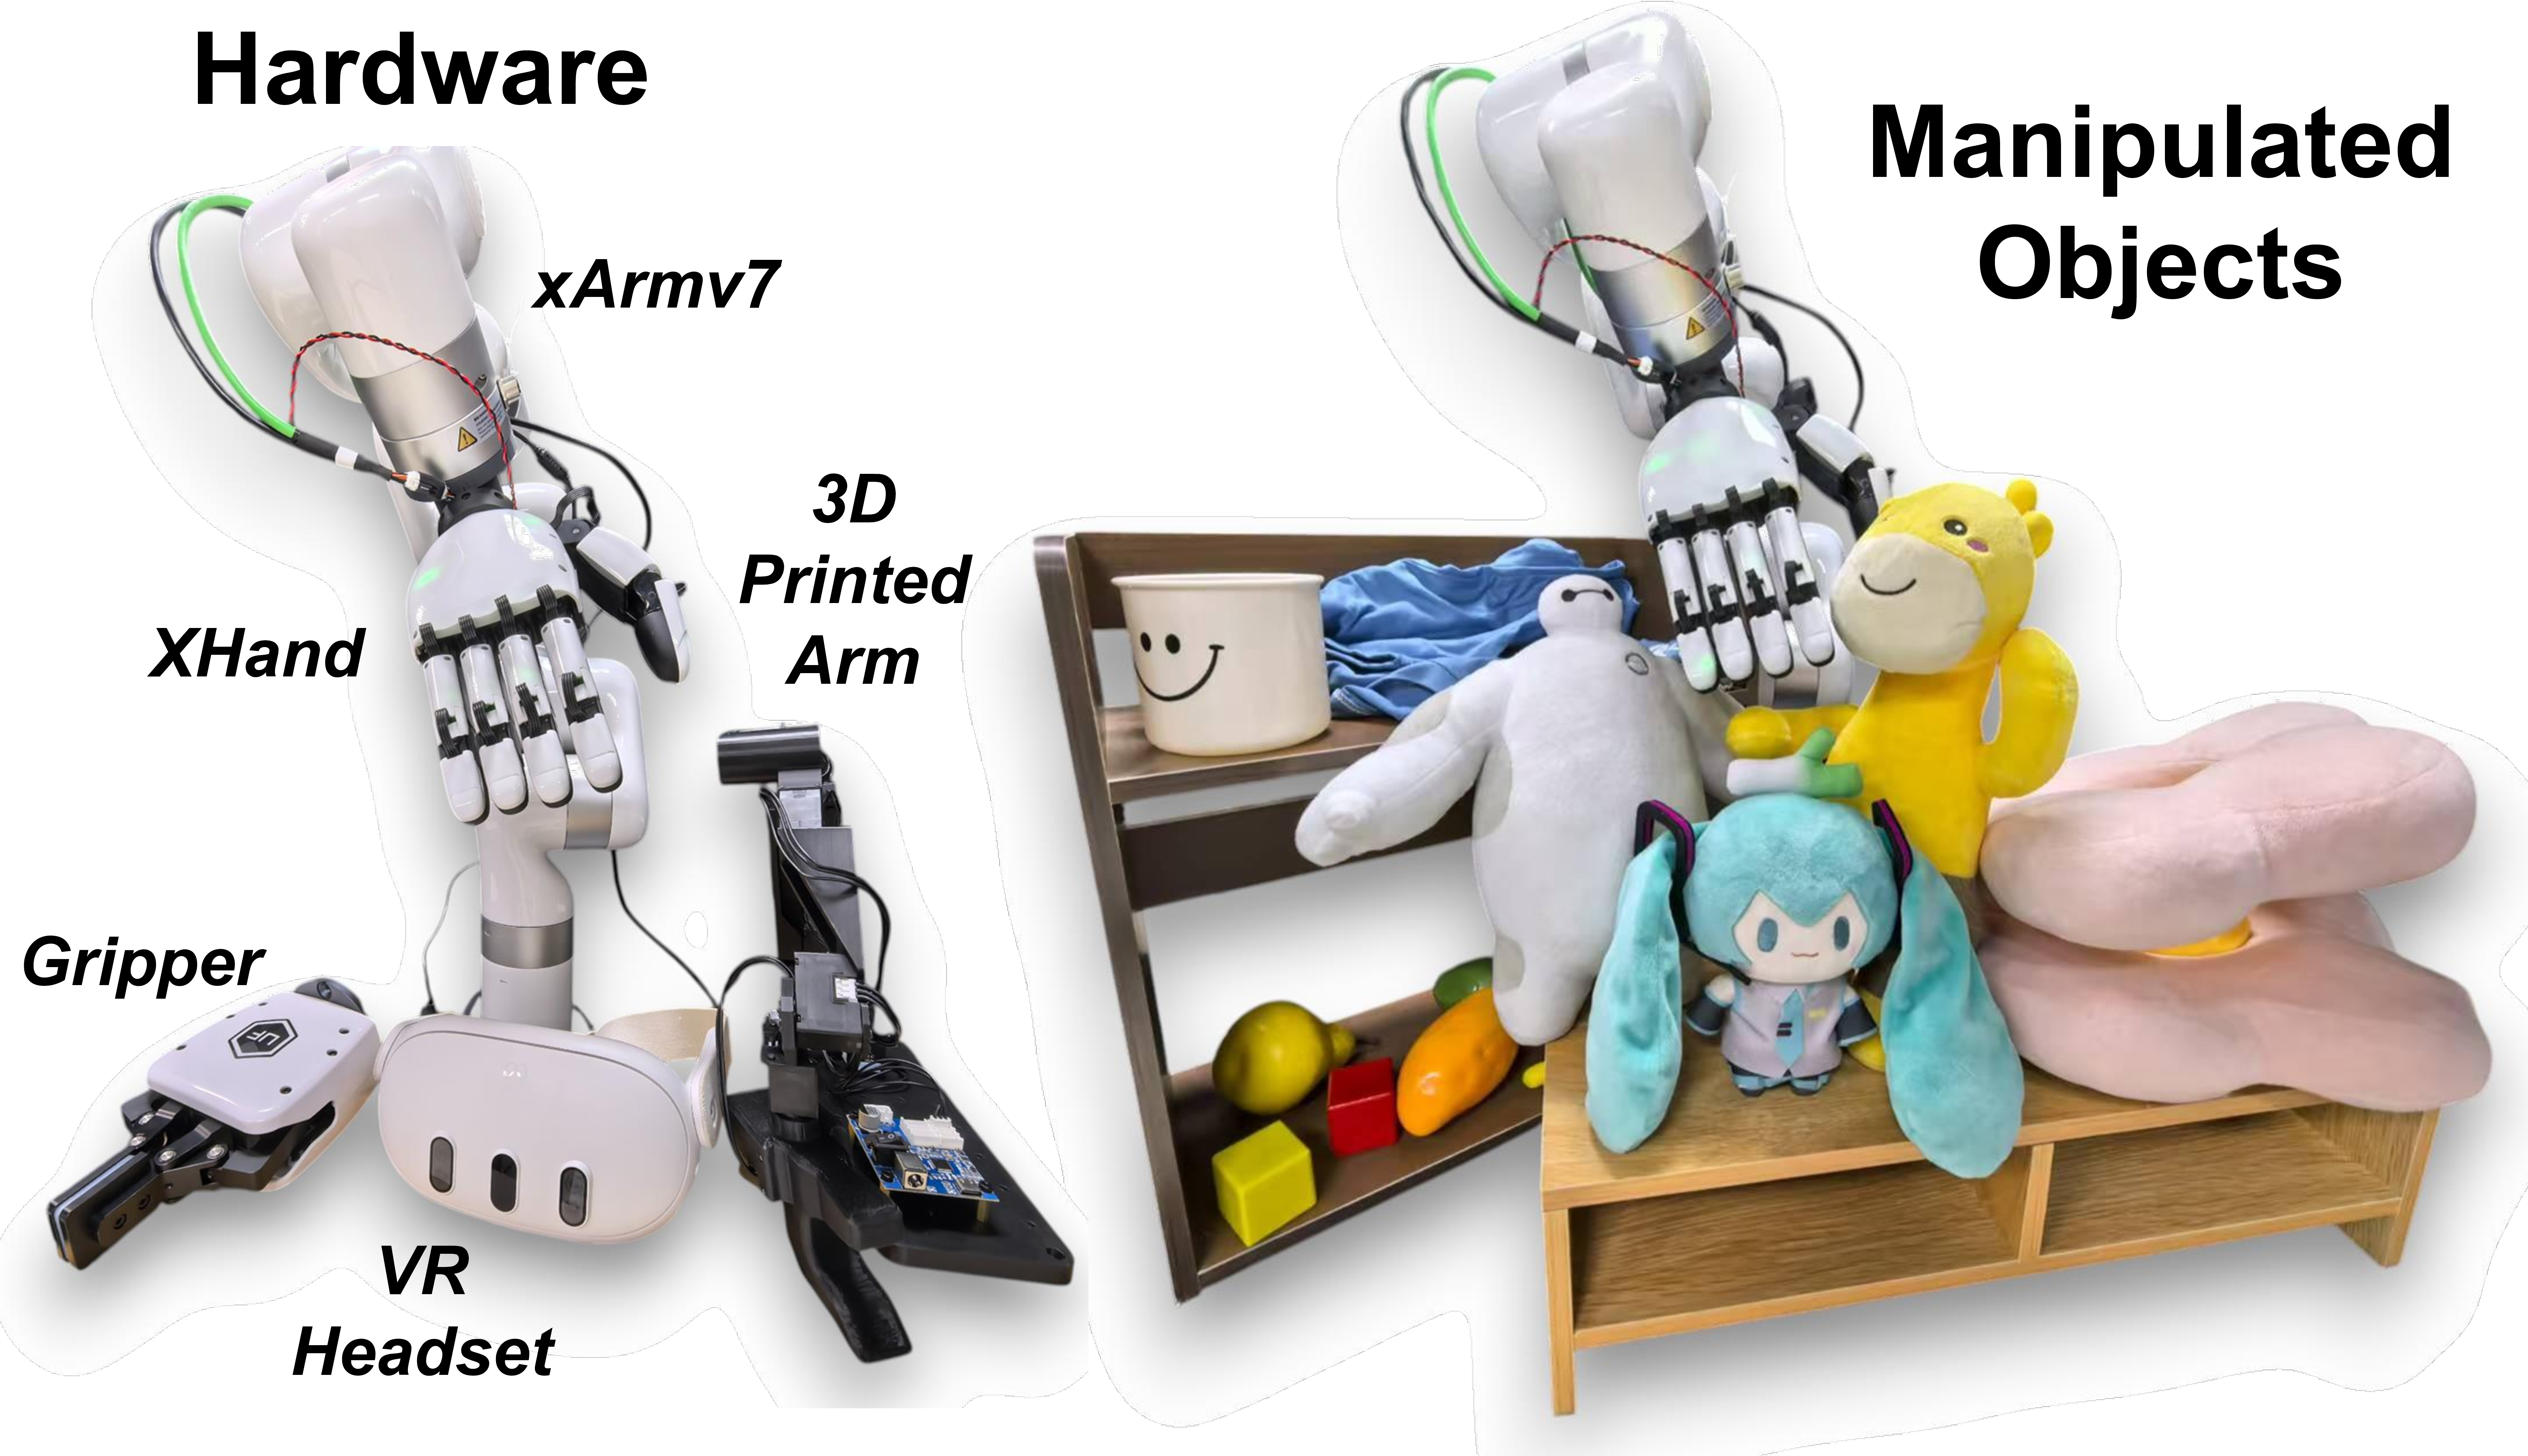
\includegraphics[width=0.99\linewidth]{pic/real_setup.pdf}
  \vspace{-8pt}
  \caption{Real-world experimental setup. 
\textbf{(a)} Our bimanual hardware setup. We collect demonstration data using a VR headset for teleoperation. 
\textbf{(b)} The set of diverse objects used in our real-world manipulation, requiring both precision and bimanual coordination.}
  \vspace{-16pt}
  \label{fig:real_setup}
\end{figure}


\noindent\textbf{Task Suite and Experimental Setup.}
We evaluate performance on 6 challenging tasks, which require both single-arm precision and complex bimanual coordination.
\begin{itemize}
    \setlength\itemsep{-0.2em}
    \item \textbf{Remove the pen cap:} A bimanual task where one hand must stabilize the pen body while the other grasps and removes the cap (Figure~\ref{fig:real_traj} (a)).
    \item \textbf{Hand over Baymax:} A coordinated bimanual task where the left hand picks up the toy and passes it to the right hand (Figure~\ref{fig:real_traj} (b)).
    \item \textbf{Push then grab box:} A long-horizon, multi-stage bimanual task. The left hand first pushes the box to the edge of a platform, after which the right hand grasps it from the table (Figure~\ref{fig:real_traj} (c)).
    \item \textbf{Place block in plate:} A single-arm task testing grasping and placement of a block into a target container.
    \item \textbf{Brush the cup:} A contact-rich bimanual task where one hand holds the cup, and the other uses a brush to perform a cleaning motion inside it.
    \item \textbf{Grasp basketball:} A bimanual task requiring the two hands to cooperatively form a stable, large-volume grasp on the ball.
\end{itemize}
\noindent Qualitative rollouts for the remaining tasks are included
in the Appendix.

\noindent\textbf{Experimental Setup.}
For each of the 6 tasks, we collect a dataset of 50 successful demonstrations. We compare three methods:
HPT~\cite{wang2024scaling} uses its publicly available pre-trained weights. We train task-specific input stems and heads for each task.
3DDP~\cite{ze20243d} is trained from scratch for each task.
\mymethod{} uses the pre-trained model.
We then fine-tune this model on the demonstrations, evaluating its ability to adapt its structural priors to the real-world domain.

\noindent\textbf{Real-World Results.}
The quantitative results are summarized in Table~\ref{tab:real_results}. Our method achieves higher success rates than all baselines across 6 tasks. This suggests that our structural action representation pre-trained on diverse data, provides a powerful prior for learning complex bimanual coordination. Figure~\ref{fig:real_traj} shows qualitative rollouts of our policy executing three of the bimanual tasks. 



\vspace{-2pt}
\subsection{Failure Case Analysis and Limitations}
\vspace{-2pt}

In addition to the quantitative ablations, we analyze failure modes which highlight the limitations of our current approach and provide avenues for future work. In complex, contact-rich bimanual tasks, one hand may severely occlude the other hand or the target object. A single, fixed camera provides no mechanism to resolve this ambiguity, starving the policy of the critical geometric information needed for precise coordination. We also observe large kinematic or contact-geometry mismatches between demonstrations and the execution platform produce action-assignment errors. These failures require explicit dynamics/force constraints or tactile closed-loop correction to resolve. We provide qualitative visualizations
of these failure modes in the Appendix.


\begin{table}[t]
\centering
\small
\resizebox{0.48\textwidth}{!}{
\begin{tabular}{l|ccc}
\toprule
  & \multicolumn{3}{c}{Success Rate} \\
 Task Description & HPT~\cite{wang2024scaling} & 3DDP~\cite{ze20243d} & \textbf{\mymethod{} (Ours)} \\
\midrule
\textit{Remove the pen cap} & 0.10 & 0.25 & {\cellcolor{tablecolor2}$\mathbf{0.30}$} \\
\textit{Hand over Baymax} & 0.50 & 0.75 & {\cellcolor{tablecolor2}$\mathbf{0.85}$} \\
\textit{Push then grab box} & 0.05 & 0.15 & {\cellcolor{tablecolor2}$\mathbf{0.35}$} \\
\textit{Place block in plate} & 0.60 & 0.85 & {\cellcolor{tablecolor2}$\mathbf{0.90}$} \\
\textit{Brush the cup} & 0.10 & 0.30 & {\cellcolor{tablecolor2}$\mathbf{0.45}$} \\
\textit{Grasp basketball} & 0.65 & 0.80 & {\cellcolor{tablecolor2}$\mathbf{0.95}$} \\
\bottomrule
\end{tabular}
}
\vspace{-8pt}
\caption{Quantitative results on 6 real-world bimanual manipulation tasks. We compare our model against baselines using in-domain demonstrations.}
\vspace{-16pt}
\label{tab:real_results}
\end{table}






